\section{Durchführung}
\label{sec:durchführung}

\subsection{Untersuchung des Spannungsrauschen von ohmschen Widerständen}

Zunächst wird das Spannungsrauschen von zwei ohmschen Widerständen untersucht.
Dazu wird die in Abbildung~\ref{fig:aufbau_einfachschaltung} gezeigte Schaltung
(Einfachschaltung) aufgebaut. Tiefpass und Gleichspannungsverstärker sind in
einem Gerät verbaut. Der Bandfilter wird auf einen Frequenzbereich
von~\SI{4}{\kilo\hertz} bis~\SI{6}{\kilo\hertz} eingestellt. Die Vorverstärkung
beträgt 1000. Die Gleichspannungsverstärkung wird konstant auf 10 eingestellt.

\begin{figure}
  \centering
  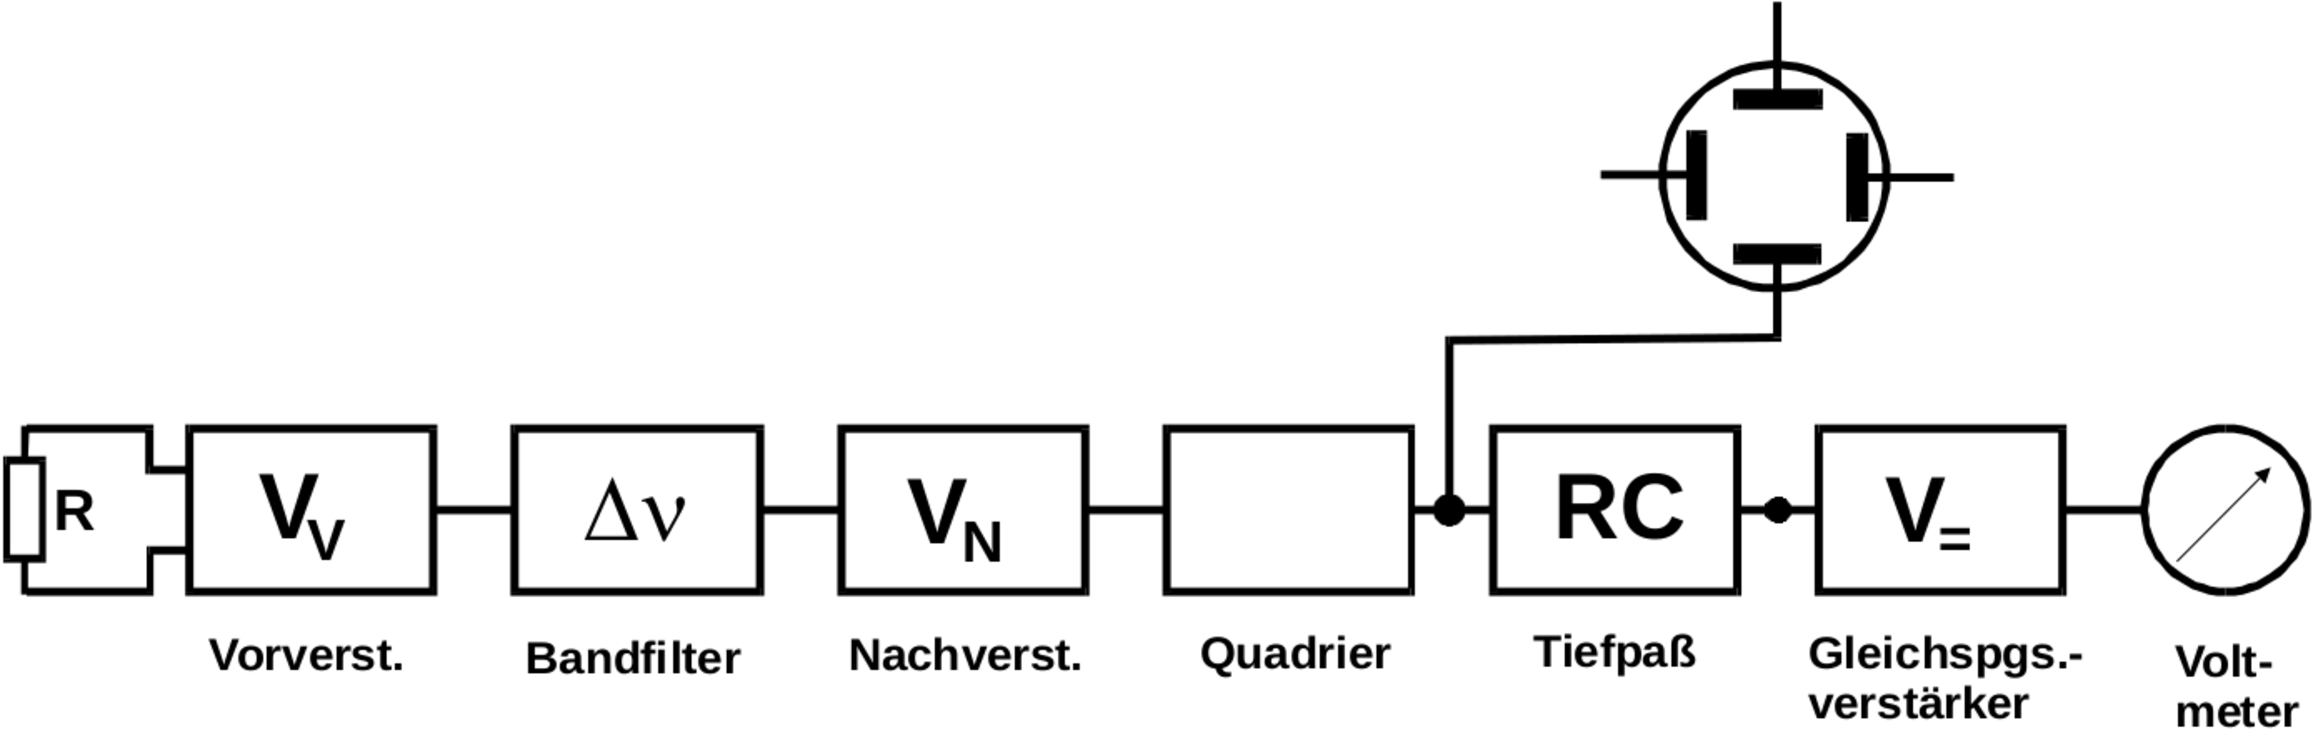
\includegraphics[width=0.9\textwidth]{figures/aufbau_einfachschaltung.pdf}
  \caption{Schematischer Aufbau der Einfachschaltung zur Messung des thermischen
  Rauschens eines ohmschen Widerstandes~\cite{V57}.}
  \label{fig:aufbau_einfachschaltung}
\end{figure}

Um das Rauschen der Widerstände korrekt bestimmen zu können, muss das
Eigenrauschen der Einfachschaltung bekannt sein. Dazu wird der Widerstand in
Abbildung~\ref{fig:aufbau_einfachschaltung} durch einen Kurzschluss ersetzt. Bei
Variation der Nachverstärkung wird nun mit Hilfe des Voltmeters die Spannung
gemessen und protokolliert.

In einem nächsten Schritt wird eine Kalibrierungskurve für den Bandfilter
aufgenommen. Dazu wird der ohmsche Widerstand durch einen Sinus-Generator
ausgetauscht. Bei Variation der eingestellten Frequenz wird wieder die Spannung
mit dem Voltmeter gemessen. Die Nachverstärkung wird hier und in allen weiteren
Versuchsteilen stets so gewählt, dass die Overload-Lampe des Quadrierers gerade
nicht bzw. nur selten aufleuchtet.

Es werden zwei variable ohmsche Widerstände untersucht. Der erste Widerstand ist
von~\SI{50}{\ohm} bis~\SI{1000}{\ohm}, der zweite Widerstand
von~\SI{1}{\kilo\ohm} bis~\SI{100}{\kilo\ohm} kontinuerlich einstellbar. Für
jeden eingestellten Widerstand wird die Spannung am Ende der Schaltung mit Hilfe
des Voltmeters gemessen. Die Widerstände selbst werden mit einem Ohmmeter
bestimmt.

Um eine vom Eigenrauschen der Schaltung weniger beeinflusste Messung durchzuführen, wird eine weitere, abgewandelte Schaltung untersucht.
Abbildung~\ref{fig:aufbau_korrelatorschaltung} zeigt den Aufbau der sogenannten
Korrelatorschaltung. Der wesentliche Unterschied besteht darin, dass das Signal
vom Widerstand ausgehend aufgespalten und durch verschiedene Verstärker und
Filter zum Quadrierer gelangt. Der Bandpass wurde zudem durch zwei
Selektivverstärker mit der Einstellung~\SI{5}{\kilo\hertz} ersetzt.

\begin{figure}
  \centering
  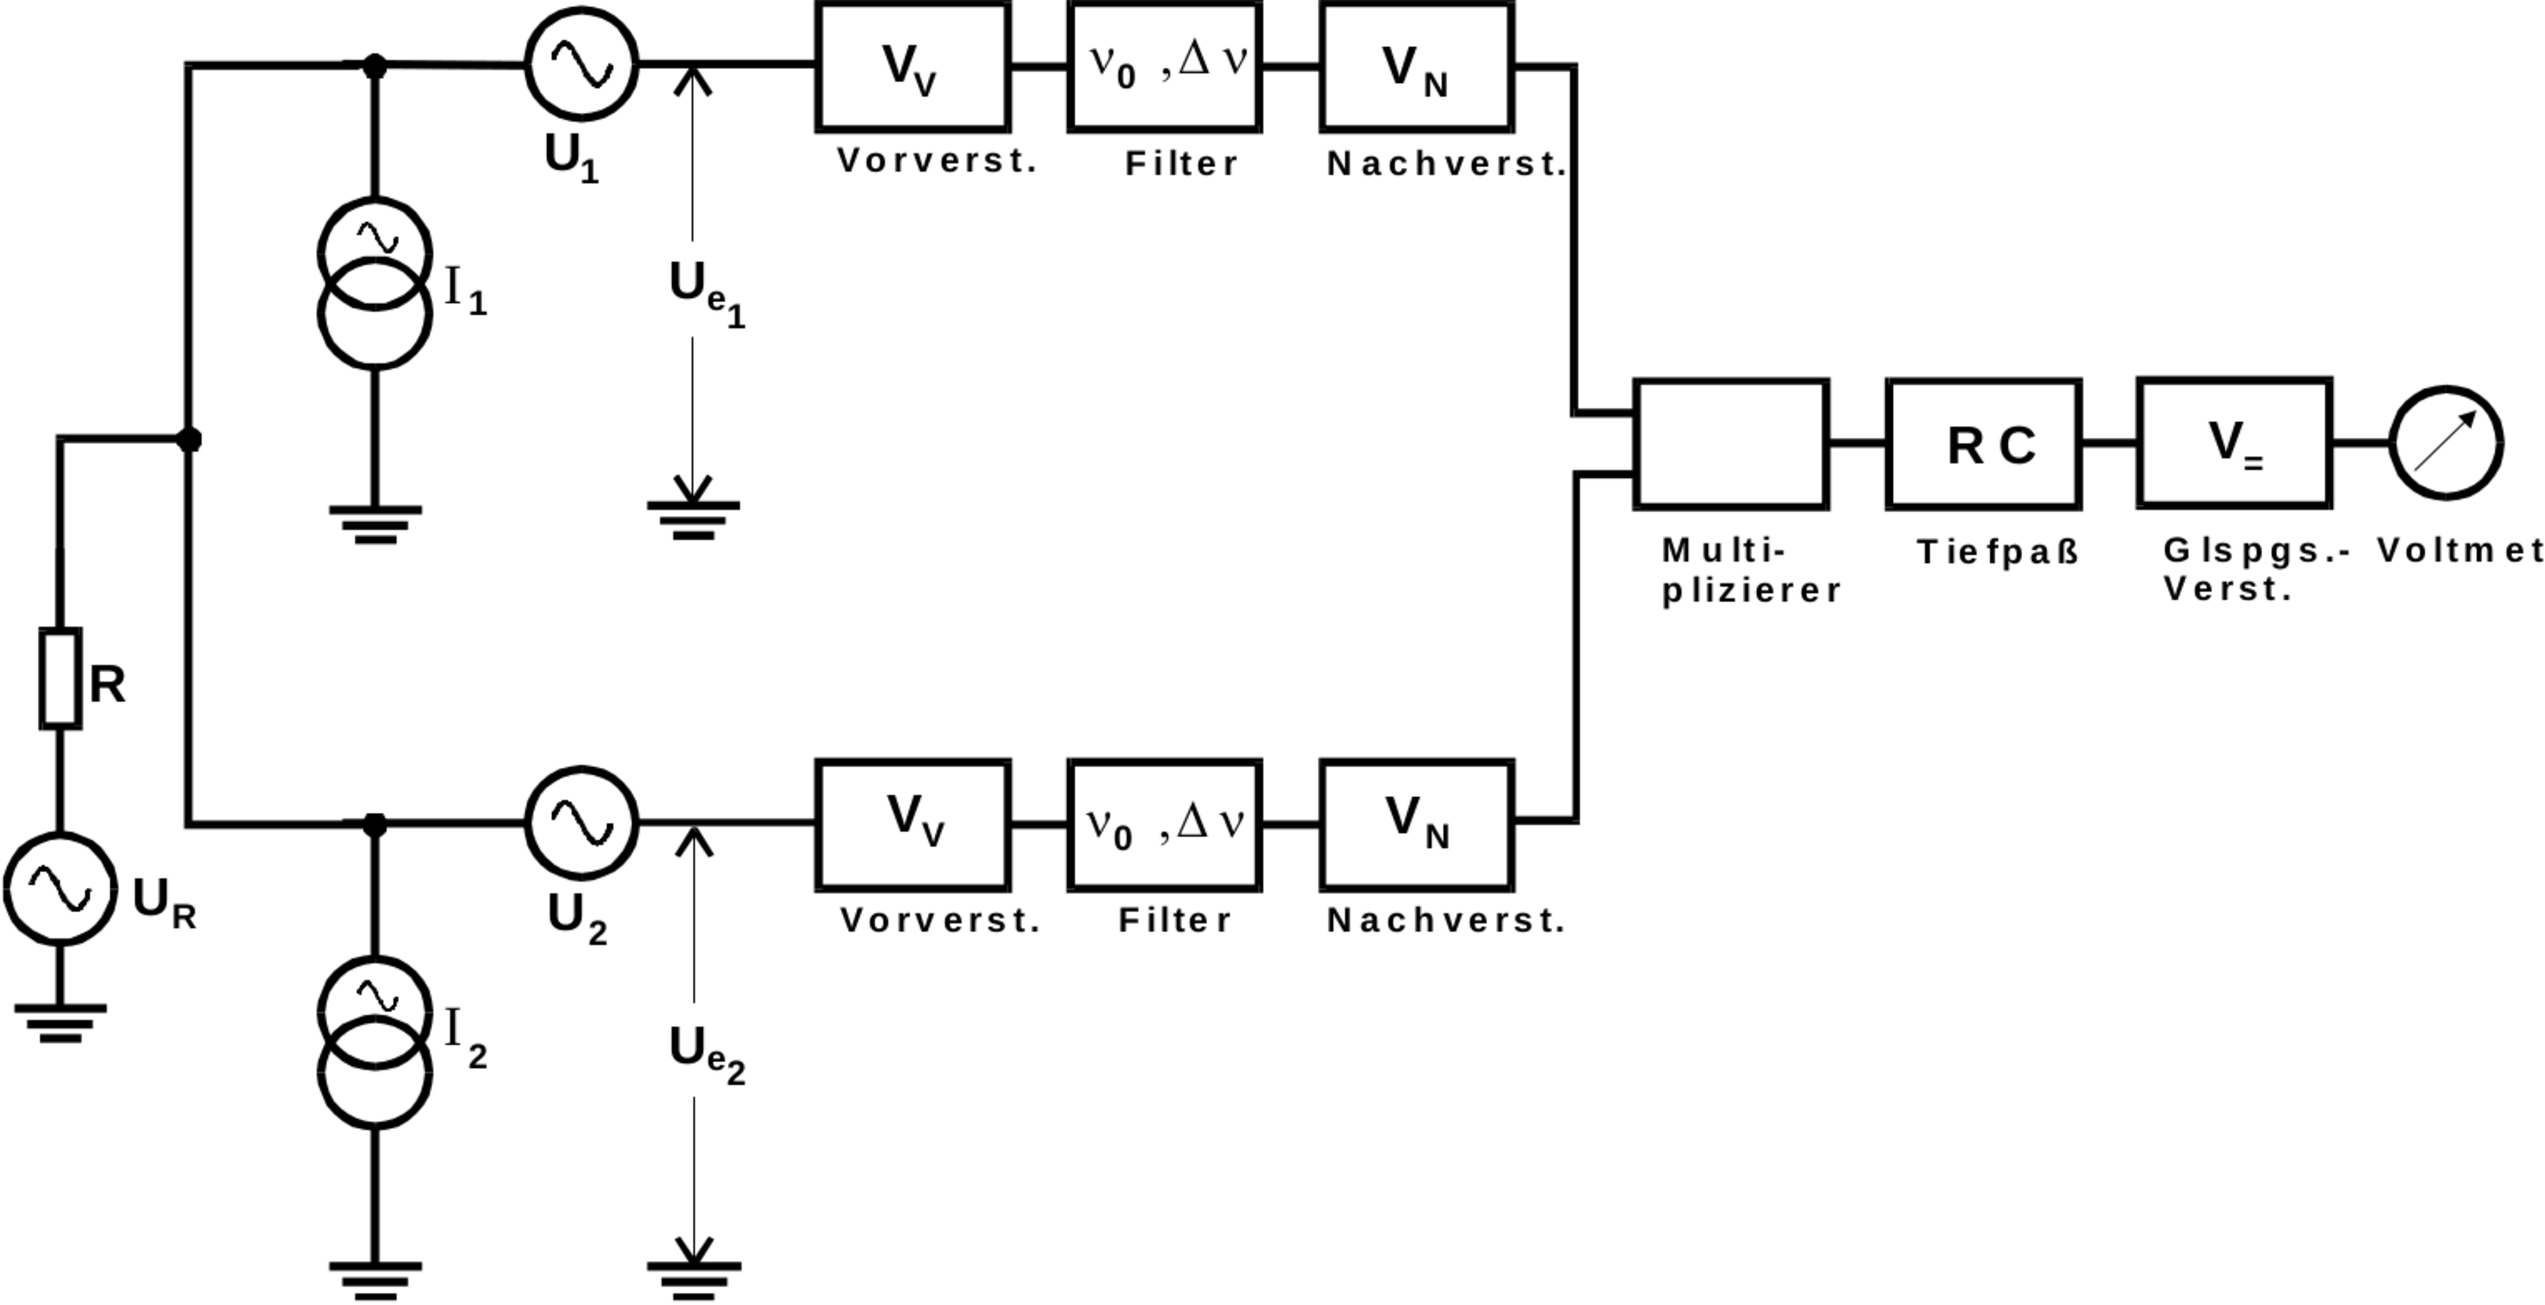
\includegraphics[width=0.9\textwidth]{figures/aufbau_korrelatorschaltung.pdf}
  \caption{Schematischer Aufbau der Korrelatorschaltung zur Messung des
  thermischen Rauschens eines ohmschen Widerstandes~\cite{V57}.}
  \label{fig:aufbau_korrelatorschaltung}
\end{figure}

Auch für diese Schaltung wird zunächst wie oben beschrieben eine
Kalibrierungskurve aufgenommen. Danach erfolgt ebenso analog eine Messreihe mit
den Widerständen.

\subsection{Untersuchung des Stromrauschens verschiedener Kathoden}

Im zweiten Versuchsabschnitt werden das Stromrauschen einer Oxydkathode sowie
einer Reinmetallkathode untersucht. Zunächst wird die Spektralverteilung der
Oxydkathode bestimmt. Dazu wird erneut die Schaltung in
Abbildung~\ref{fig:aufbau_einfachschaltung} aufgebaut. Anstelle des Widerstandes
wird nun allerdings der Ausgang der Oxydkathode angeschlossen, an dem die
Spannung über dem Arbeitswiderstand der Kathode abgegriffen werden kann. Je nach
betrachtetem Frequenzbereich wird entweder der Bandpass oder ein
Selektivverstärker als Filter verwendet. Bei der Oxydkathode ist es wichtig zu
beachten, dass diese nicht im Sättigungsbereich betrieben werden darf, um sie
nicht zu beschädigen. In einer Messreihe wird die Spannung in Abhängigkeit von
der am Bandpass oder Selektivverstärker eingestellten Frequenz aufgenommen.

Als nächstes wird die Reinmetallkathode betrachtet. Diese soll im
Sättigungsbereich betrieben werden. Um herauszufinden, ab wann sich die Kathode
in diesem Bereich befindet, wird der Anodenstrom in Abhängigkeit von der
Anodenspannung bei verschiedenen konstanten Heizströmen gemessen. Sobald sich
der Strom bei Erhöhung der Spannung nicht mehr ändert, ist der Betrieb erreicht.
Zuletzt wird wie bei der Oxydkathode das Frequenzspektrum aufgenommen.
